\def\duedate{\today}
\def\HWnum{7}
\documentclass[10pt,a4paper]{book}

% custom section formatting
\usepackage{titlesec}
\titleformat{\chapter}[display]
{\normalfont\Large\filcenter\sffamily}
{\titlerule[1pt]%
\vspace{1pt}%
\titlerule
\vspace{1pc}%
\LARGE\MakeUppercase{\chaptertitlename} \thechapter}
{1pc}
{\titlerule
\vspace{1pc}%
\Huge}

% appendix handling
\usepackage[toc,page]{appendix}
    
% encoding for file and font
\usepackage[utf8]{inputenc}
\usepackage[T1]{fontenc}

% math formatting/tools
\usepackage{amsmath}
\usepackage{amssymb}
\usepackage{mathtools}
\usepackage[arrowdel]{physics}

% unit formatting
\usepackage{siunitx}
\AtBeginDocument{\RenewCommandCopy\qty\SI}

% figure formatting/tools
\usepackage{graphicx}
\usepackage{float}
\usepackage{subcaption}
\usepackage{multirow}
\usepackage{import}
\usepackage{pdfpages}
\usepackage{transparent}
\usepackage{currfile}

\NewDocumentCommand\incfig{O{1} m}{
    \def\svgwidth{#1\textwidth}
    \import{./Figures/\currfiledir}{#2.pdf_tex}
}

\newcommand{\bef}{\begin{figure}[h!tb]\centering}
\newcommand{\eef}{\end{figure}}

\newcommand{\bet}{\begin{table}[h!tb]\centering}
\newcommand{\eet}{\end{table}}

% hyperlink references 
\usepackage{hyperref}
\hypersetup{
    colorlinks=true,
    linkcolor=blue,
    filecolor=magenta,
    urlcolor=cyan,
    pdftitle={Physics 1 Notes},
    pdfauthor={Richard Whitehill},
    pdfpagemode=FullScreen
}
\urlstyle{same}

\newcommand{\eref}[1]{Eq.~(\ref{eq:#1})}
\newcommand{\erefs}[2]{Eqs.~(\ref{eq:#1})--(\ref{eq:#2})}

\newcommand{\fref}[1]{Fig.~(\ref{fig:#1})}
\newcommand{\frefs}[2]{Fig.~(\ref{fig:#1})--(\ref{fig:#2})}

\newcommand{\aref}[1]{Appendix~(\ref{app:#1})}
\newcommand{\sref}[1]{Section~(\ref{sec:#1})}
\newcommand{\srefs}[2]{Sections~(\ref{sec:#1})-(\ref{sec:#2})}

\newcommand{\tref}[1]{Table~(\ref{tab:#1})}
\newcommand{\trefs}[2]{Table~(\ref{tab:#1})--(\ref{tab:#2})}

% tcolorbox formatting/definitions
\usepackage[most]{tcolorbox}
\usepackage{xcolor}
\usepackage{xifthen}
\usepackage{parskip}

\definecolor{peach}{rgb}{1.0,0.8,0.64}

\DeclareTColorBox[auto counter, number within=chapter]{defbox}{O{}}{
    enhanced,
    boxrule=0pt,
    frame hidden,
    borderline west={4pt}{0pt}{green!50!black},
    colback=green!5,
    before upper=\textbf{Definition \thetcbcounter \ifthenelse{\isempty{#1}}{}{: #1} \\ },
    sharp corners
}

\newcommand*{\eqbox}{\tcboxmath[
    enhanced,
    colback=black!10!white,
    colframe=black,
    sharp corners,
    size=fbox,
    boxsep=8pt,
    boxrule=1pt
]}

\newtcolorbox[auto counter, number within=chapter]{exbox}{
    parbox=false,
    breakable,
    enhanced,
    sharp corners,
    boxrule=1pt,
    colback=white,
    colframe=black,
    before upper= \textbf{Example \thetcbcounter:}\,,
    before lower= \textbf{Solution:}\,,
    segmentation hidden
}

\newtcolorbox{resbox}{
    enhanced,
    colback=black!10!white,
    colframe=black,
    boxrule=1pt,
    boxsep=0pt,
    top=2pt,
    ams nodisplayskip,
    sharp corners
}


\begin{document}

\prob{1}{

Two concentric spheres have radii $a,b$ ($b > a$) and each is divided into two hemispheres by the same horizontal plane.
The upper hemisphere of the inner sphere and the lower hemisphere of the outer sphere are maintained at potential $V$.
The other hemispheres are at zero potential.

(a) Determine the potential in the region $a \leq r \leq b$ as a series in Legendre polynomials.
include terms at least up to $l=4$.
Check your solution against known results in the limiting cases $b \rightarrow \infty$ and $a \rightarrow \infty$.

(b) Solve for the potential using the appropriate Green function, and verify that the answer obtained in this way agrees with the direct solution in part (a) obtained from the differential equation.

}

\sol{

(a) We solved this problem in the previous homework, so we will skip the derivations and just quote the results here for brevity:
\begin{eqnarray}
\begin{aligned}
    \Phi(r,\theta) = \frac{V}{2} \Bigg( 1 + \sum_{l=0}^{\infty} \frac{ P_{2l}(0) - P_{2(l+1)}(0) }{ a^{4l+3} - b^{4l+3} } &\Big[ ( a^{2(l+1)} + b^{2(l+1)} ) r^{2l+1} \\
                                                                                                                          &- a^{2(l+1)}b^{2(l+1)} (a^{2l+1} + b^{2l+1}) r^{-2(l+1)} \Big] \Bigg)
.\end{aligned}
\end{eqnarray}
\begin{eqnarray}
\begin{aligned}
    \Phi(r,\theta) &= \frac{V}{2} \Bigg\{ 1 + \frac{3}{2} \frac{(a^2-b^2)r - a^2b^2(a+b)r^{-2}}{a^3-b^3} P_{1}(\cos{\theta}) \\
                   &- \frac{7}{8} \frac{(a^{4} - b^{4})r^{3} - a^{4}b^{4}(a^3 + b^3) r^{-4}}{a^{7} - b^{7}} P_{3}(\cos{\theta}) + \ldots \Bigg\}
.\end{aligned}
\end{eqnarray}
Refer to problem 1 of HW 6 for details.

(b) Since we are given the potential on the surfaces of the spheres, we can construct a Green function such that $G(\va*{x},\va*{x}') = 0$ if $|\va*{x}'| = a,b$.
We could do this via the method of images.
The procedure would look something like this.
First, we would place an image charge outside the sphere $b$ to cancel the potential on the outside sphere produced by the charge between the spheres.
Similarly, we would place an image charge inside the sphere $a$ to cancel the potential on the inner sphere produced by the charge between the spheres.
Notice though that the potential produced by the image charge beyond the outer sphere $b$ produces a nonzero potential on the inner sphere, meaning we would have to place another image charge to cancel this contribution, and via a similar reason, we would have to place an image charge beyond the outer sphere to cancel the potential produced by the image charge inside the inner sphere.
This line of reasoning would continue \textit{ad infinitum}.

While we could construct the series and attempt to evaluate it, it is much likely easier to solve for the Green's function directly as
\begin{eqnarray}
    g_{l}(r,r') = C y_1(r_{<}) y_2(r_{>})
.\end{eqnarray}
Actually, we have already done so in class, yielding
\begin{eqnarray}
    g_{l}(r,r') = \frac{4\pi}{2l+1} \Big[ 1 - \Big( \frac{a}{b} \Big)^{2l+1} \Big]^{-1} \Big( r_{<}^{l} - \frac{a^{2l+1}}{r_{<}^{l+1}} \Big) \Big( \frac{1}{r_{>}^{l+1}} - \frac{r_{>}^{l}}{b^{2l+1}} \Big)
.\end{eqnarray}
The general Green's function
\begin{eqnarray}
    G(\va*{x},\va*{x}') = \sum_{l=0}^{\infty} \sum_{m=-l}^{l} g_{l}(r,r') Y_{lm}^{*}(\theta',\phi') Y_{lm}(\theta,\phi)
.\end{eqnarray}
The potential is then
\begin{eqnarray}
    \Phi(\va*{x}) = -\frac{1}{4\pi} \int_{S = \partial V} \dd{S'} \Phi(\va*{x}') \pdv{G}{n'}
.\end{eqnarray}

When $r_{>} = r'$, we have
\begin{eqnarray}
    G(\va*{x},\va*{x}') = \sum_{l=0}^{\infty} \sum_{m=-l}^{l} \frac{4 \pi}{2l+1} \Big[ 1 - \frac{a^{2l+1}}{b^{2l+1}} \Big]^{-1} \Big( r^{l} - \frac{a^{2l+1}}{r^{l+1}} \Big) \Big( \frac{1}{r'^{l+1}} - \frac{r'^{l}}{b^{2l+1}} \Big) Y_{lm}^{*}(\theta',\phi') Y_{lm}(\theta,\phi)
\end{eqnarray}
which gives at the outer surface where $r' = b$
\begin{eqnarray}
\begin{aligned}
    - \frac{1}{4\pi} \pdv{G}{n'}\Big|_{r'=b} &= -\frac{1}{4 \pi} \pdv{G}{r'}\Big|_{r'=b} \\
                                             &= \sum_{l=0}^{\infty} \sum_{m=-l}^{l} \frac{b^{l-1}}{b^{2l+1} - a^{2l+1}} \Big( r^{l} - \frac{a^{2l+1}}{r^{l+1}} \Big) Y_{lm}^{*}(\theta',\phi') Y_{lm}(\theta,\phi)
.\end{aligned}
\end{eqnarray}
The contribution from the surface $r = b$ is then
\begin{eqnarray}
    \Phi_{b} = \sum_{l=0}^{\infty} \sum_{m=-l}^{l} \frac{b^{l-1}}{b^{2l+1} - a^{2l+1}} \Big( r^{l} - \frac{a^{2l+1}}{r^{l+1}} \Big) Y_{lm}(\theta,\phi) \int b^2 \dd{\Omega'} V \Theta(\theta - \pi/2) Y^{*}_{lm}(\theta',\phi')
,\end{eqnarray}
where $\Theta(x)$ is the Heaviside step-function.
Notice that since the potential at the surface is independent of $\phi$, only the $m = 0$ term contributes (as expected since the problem is azimuthally symmetric) and
\begin{eqnarray}
\begin{aligned}
    \Phi_{b} &= \sum_{l=0}^{\infty} \frac{b^{l+1}}{b^{2l+1} - a^{2l+1}} \Big( r^{l} - \frac{a^{2l+1}}{r^{l+1}} \Big) \sqrt{ \frac{2l+1}{4\pi} } P_{l}(\cos{\theta}) V (2\pi) \sqrt{\frac{2l+1}{4 \pi}} \int_{-1}^{0} P_{l}(\cos{\theta}) \dd{(\cos{\theta})} \\
             &= \frac{V}{2} \sum_{l=0}^{\infty} [ P_{l+1}(0) - P_{l-1}(0) ] \frac{b^{l+1}}{b^{2l+1} - a^{2l+1}} \Big( r^{l} - \frac{a^{2l+1}}{r^{l+1}} \Big) P_{l}(\cos{\theta})
.\end{aligned}
\end{eqnarray}
Note that we define $P_{-1}(0) = -1$ as in the previous homework such that we can include the $l = 0$ term implicitly.

Similarly, we can determine the contribution from the sphere at $r = a$.
The Green function when $r_{<} = r'$ is given by
\begin{eqnarray}
    G(\va*{x},\va*{x}') = \sum_{l=0}^{\infty} \sum_{m=-l}^{l} \frac{4\pi}{2l+1} \Big[ 1 - \frac{a^{2l+1}}{b^{2l+1}} \Big]^{-1} \Big( r'^{l} - \frac{a^{2l+1}}{r'^{l+1}} \Big) \Big( \frac{1}{r^{l+1}} - \frac{r^{l}}{b^{2l+1}} \Big) Y_{lm}^{*}(\theta',\phi') Y_{lm}(\theta,\phi)
,\end{eqnarray}
and therefore
\begin{eqnarray}
\begin{aligned}
    -\frac{1}{4\pi} \pdv{G}{n'}\Big|_{r'=a} &= \frac{1}{4\pi} \pdv{G}{r'}\Big|_{r'=a} \\
                                            &= \sum_{l=0}^{\infty} \sum_{m=-l}^{l} a^{l-1} \Big[ 1 - \frac{a^{2l+1}}{b^{2l+1}} \Big]^{-1} \Big( \frac{1}{r^{l+1}} - \frac{r^{l}}{b^{2l+1}} \Big) Y_{lm}^{*}(\theta',\phi') Y_{lm}(\theta,\phi)
.\end{aligned}
\end{eqnarray}
The contribution
\begin{eqnarray}
    \Phi_{a} = \frac{V}{2} \sum_{l=0}^{\infty} [ P_{l-1}(0) - P_{l+1}(0) ] \frac{a^{l+1}}{b^{2l+1} - a^{2l+1}} \Big( \frac{b^{2l+1}}{r^{l+1}} - r^{l} \Big) P_{l}(\cos{\theta})
.\end{eqnarray}
Summing these gives the total potential due to both surface contributions as
\begin{eqnarray}
\eqbox{
\begin{aligned}
    \Phi(\va*{x}) &= \frac{V}{2} \sum_{l=0}^{\infty} \frac{P_{l-1}(0) - P_{l+1}(0)}{b^{2l+1} - a^{2l+1}} \Bigg\{ a^{l+1} \Big( \frac{b^{2l+1}}{r^{l+1}} - r^{l} \Big) + b^{l+1} \Big( \frac{a^{2l+1}}{r^{l+1}} - r^{l} \Big) \Bigg\} \\
                  &= \frac{V}{2} \sum_{l=0}^{\infty} \frac{P_{l+1}(0) - P_{l-1}(0)}{b^{2l+1} - a^{2l+1}} \Bigg\{ [a^{l+1} + b^{l+1}] r^{l} - a^{l+1} b^{l+1} [a^{l+1} + b^{l+1}] r^{-(l+1)} \Bigg\} \\
                  &= \frac{V}{2} \Bigg[ 1 + \sum_{l=0}^{\infty} \frac{P_{2(l+1)}(0) - P_{2l}(0)}{b^{4l+3} - a^{4l+3}} \Bigg\{ [a^{2(l+1)} + b^{2(l+1)}] r^{2l+1} - \frac{a^{2(l+1)} b^{2(l+1)} [a^{2l+1} + b^{2l+1}]}{r^{2(l+1)}} \Bigg\} \Bigg]
,\end{aligned}
}
\end{eqnarray}
which agrees with our original result, derived directly as a series in Legendre polynomials.

}


\prob{2}{

Consider the Green function appropriate for Neumann boundary conditions for the volume $V$ between the concentric spherical surfaces defined by $r = a$ and $r = b$, ($a < b$).
To be able to use Eq. (1.46)
\begin{eqnarray}
    \Phi(\va*{x}) = \expval{\Phi}_{S} + \frac{1}{4 \pi \epsilon_0} \int_{V} \rho(\va*{x}') G_{N}(\va*{x},\va*{x}') \dd[3]{\va*{x}'} + \frac{1}{4 \pi} \oint_{S} \pdv{\Phi(\va*{x}')}{n'} G_{N} \dd{S'}
.\end{eqnarray}
from \textit{Jackson textbook} for the potential, impose the simple constraint (1.45)
\begin{eqnarray}
    \label{eq:neumann-BC}
    \pdv{G_{N}}{n'}(\va*{x},\va*{x}') = -\frac{4 \pi}{S}~{\rm for}~\va*{x}' \in S
\end{eqnarray}
given in \textit{Jackson textbook}.
Use an expansion in spherical harmonics of the form,
\begin{eqnarray}
    G(\va*{x},\va*{x}') = \sum_{l=0}^{\infty} g_{l}(r,r') P_{l}(\cos{\gamma})
,\end{eqnarray}
where $g_{l}(r,r') = r_{<}^{l}/r_{>}^{l+1} + f_{l}(r,r')$.

(a) Show that for $l > 0$, the radial Green function has the symmetric form
\begin{eqnarray}
    g_{l}(r,r') = \frac{r_{<}^{l}}{r_{>}^{l+1}} + \frac{1}{b^{2l+1} - a^{2l+1}} \Bigg[ \frac{l+1}{l} (r r')^{l} + \frac{l}{l+1} \frac{(ab)^{2l+1}}{(rr')^{l+1}} + a^{2l+1} \Big( \frac{r^{l}}{r'^{l+1}} + \frac{r'^{l}}{r^{l+1}} \Big) \Bigg]
.\end{eqnarray}

(b) Show that for $l = 0$
\begin{eqnarray}
    g_{0}(r,r') = \frac{1}{r_{>}} - \Big( \frac{a^2}{a^2 + b^2} \Big) \frac{1}{r'} + f(r)
,\end{eqnarray}
where $f(r)$ is arbitrary.
Show explicitly in (1.46) in \textit{Jackson textbook} that answers for the potential $\Phi(\va*{x})$ are independent of $f(r)$.
[The arbitariness in the Neumann Green function can be removed by symmetrizing $g_0$ in $r$ and $r'$ with a suitable choice of $f(r)$.]

}

\sol{

(a) Note that $S = 4\pi(a^2+b^2)$ is the total surface area over both spheres.
Observe that the form of $g_{l}$ is given in such a way that the first term satisfies the inhomogeneous equation for the radial part of Laplace's equation (i.e. $\mathcal{L}_{r} g_{l}(r,r') \sim \delta(r-r')$), and the second term $f_{l}$ is some solution of the homogeneous equation, chosen such that the boundary condition \eref{neumann-BC} is satisfied.
We already know the generic homogeneous solution:
\begin{eqnarray}
    f_{l}(r,r') = A_{l}(r) r'^{l} + B_{l}(r) r'^{-l-1}
,\end{eqnarray}

We can determine the conditions that $A_{l}$ and $B_{l}$ must satisfy generally as follows:
\begin{eqnarray}
    \pdv{G_{N}}{n'}\Big|_{r' = R} = \sum_{l=0}^{\infty} \pdv{g_{l}(r,r')}{n'}\Big|_{r'=R} P_{l}(\cos{\gamma}) = -\frac{1}{a^2 + b^2}
,\end{eqnarray}
where $R$ is either $a$ or $b$.
Exploiting the orthogonality of the Legendre polynomials we have
\begin{eqnarray}
    \pdv{g_{l}(r,r')}{n'}\Big|_{r'=R} = -\frac{\delta_{l 0}}{a^2 + b^2}
.\end{eqnarray}
This gives the two boundary conditions
\begin{align}
    \pdv{g_{l}(r,r')}{r'}\Big|_{r'=a} = \frac{\delta_{l 0}}{a^2 + b^2} ~{\rm and}~ \pdv{g_{l}(r,r')}{r'}\Big|_{r'=b} = -\frac{\delta_{l 0}}{a^2 + b^2}
.\end{align}
The derivatives are as follows:
\begin{align}
    \pdv{g_{l}(r,r')}{r'}\Big|_{r'=a} &= l \frac{a^{l-1}}{r^{l+1}} + lA_{l} a^{l-1} - (l+1) B_{l} a^{-l-2} \\
    \pdv{g_{l}(r,r')}{r'}\Big|_{r'=b} &= -(l+1) \frac{r^{l}}{b^{l+2}} + l A_{l} b^{l-1} - (l+1) B_{l} b^{-l-2}
.\end{align}

Focusing on the $l>0$ contributions, these expressions are set to zero, giving
\begin{align}
    l a^{2l+1} A_{l} - (l+1) B_{l} = -\frac{l a^{2l+1}}{r^{l+1}} \\
    l b^{2l+1} A_{l} - (l+1) B_{l} = (l+1) r^{l}
.\end{align}
Solving for $A_{l}$ gives
\begin{eqnarray}
    l(b^{2l+1} - a^{2l+1}) A_{l} = (l+1) r^{l} + \frac{la^{2l+1}}{r^{l+1}} \Rightarrow A_{l} = \frac{1}{l} \frac{(l+1) r^{l} + la^{2l+1} r^{-l-1}}{b^{2l+1} - a^{2l+1}}
,\end{eqnarray}
and
\begin{eqnarray}
    B_{l} = \frac{1}{(l+1)} \frac{(l+1) a^{2l+1} r^{l} + l a^{2l+1} b^{2l+1} r^{-l-1}}{b^{2l+1} - a^{2l+1}}
.\end{eqnarray}
We then have for $l > 0$
\begin{eqnarray}
\eqbox{
\begin{aligned}
    g_{l}(r,r') &= \frac{r_{<}^{l}}{r_{>}^{l+1}} + \frac{1}{b^{2l+1} - a^{2l+1}} \Bigg[ \Big( \frac{l+1}{l} r^{l} + \frac{a^{2l+1}}{r^{l+1}} \Big) r'^{l} + \Big( a^{2l+1} r^{l} + \frac{l}{l+1} \frac{a^{2l+1}b^{2l+1}}{r^{l+1}} \Big) \frac{1}{r'^{l+1}} \Bigg] \\
                &= \frac{r_{<}^{l}}{r_{>}^{l+1}} + \frac{1}{b^{2l+1} - a^{2l+1}} \Bigg[ \frac{l+1}{l} (r r')^{l} + \frac{l}{l+1} \frac{(ab)^{2l+1}}{(r r')^{l+1}} + a^{2l+1} \Bigg( \frac{r^{l}}{r'^{l+1}} + \frac{r'^{l}}{r^{l+1}} \Bigg) \Bigg]
.\end{aligned}
}
\end{eqnarray}

(b) If we now consider $l = 0$ we have the system
\begin{align}
    -\frac{B_{0}}{a^2} &= \frac{1}{a^2 + b^2} \\
    -\frac{1}{b^2} - \frac{B_{0}}{b^2} &= -\frac{1}{a^2 + b^2}
.\end{align}
These are redundant equations and give $B_{0} = -a^2/(a^2 + b^2)$.
Note that $A_{0} = f(r)$ is undetermined by our BCs, giving
\begin{eqnarray}
    \eqbox{
    g_{0}(r,r') = \frac{1}{r_{>}} - \frac{a^2}{a^2 + b^2} \frac{1}{r'} + f(r)
}
.\end{eqnarray}

Note that this arbitrary function does not contribute to the potential:
\begin{eqnarray}
    \frac{1}{4 \pi \epsilon_0} \int_{V} \rho(\va*{x}') f(r) + \frac{1}{4\pi} \oint_{S} \pdv{\Phi(\va*{x}')}{n'} f(r) = \frac{1}{4\pi} f(r) \Bigg[ \frac{Q}{\epsilon_0} - \oint_{S} \va*{E}(\va*{x}') \cdot \dd{\va*{S}'} \Bigg] = 0
,\end{eqnarray}
relating the two terms via Gauss's law.

}


\prob{3}{

Apply the Neumann Green function of Problem 2 to the situation in which the normal electric field is $E_{r} = -E_0 \cos{\theta}$ at the outer surface ($r = b$) and is $E_{r} = 0$ on the inner surface ($r = a$).

(a) Show that the electrostatic potential inside the volume $V$ is
\begin{eqnarray}
    \Phi(\va*{x}) = E_0 \frac{r \cos{\theta}}{1 - p^3} \Big( 1 + \frac{a^3}{2 r^3} \Big)
,\end{eqnarray}
where $p = a/b$.
Find the components of the electric field,
\begin{eqnarray}
    E_{r}(r,\theta) = -E_0 \frac{\cos{\theta}}{1 - p^3} \Big( 1 - \frac{a^3}{r^3} \Big), \quad E_{\theta}(r,\theta) = E_0 \frac{\sin{\theta}}{1 - p^3} \Big( 1 + \frac{a^3}{2r^3} \Big)
.\end{eqnarray}

(b) Calculate the Cartesian or cylindrical components of the field, $E_{z}$ and $E_{\rho}$, and make a sketch or computer plot of the lines of electric force for a typical case of $p = 0.5$.

}

\sol{

The BCs are given here as
\begin{eqnarray}
    \pdv{\Phi}{r}\Big|_{r = a} = 0 \quad{\rm and}\quad \pdv{\Phi}{r}\Big|_{r=b} = E_0 \cos{\theta}
.\end{eqnarray}
Thus, the potential (assuming no sources), neglecting the average over the surface since this constant is not physically relevant,
\begin{eqnarray}
\begin{aligned}
    \Phi(\va*{x}) &= \frac{1}{4 \pi} \int_{S_{b}} E_0 \cos{\theta'} \sum_{l=0}^{\infty} \sum_{m=-l}^{l} g_{l}(r,b) \Bigg[ \frac{4 \pi}{2l+1} Y_{lm}^{*}(\theta',\phi') Y_{lm}(\theta,\phi) \Bigg] \dd{S'} \\
                  &= E_0 \sum_{l=0}^{\infty} \sum_{m=-l}^{l} \frac{b^2}{2l+1} g_{l}(r,b) Y_{lm}(\theta,\phi) \int Y_{lm}^{*}(\theta',\phi') P_{1}(\cos{\theta'}) \dd{\Omega'} \\
                  &= \frac{1}{2} E_0 b^2 \sum_{l=0}^{\infty} g_{l}(r,b) P_{l}(\cos{\theta}) \int_{-1}^{1} P_{l}(\cos{\theta}') P_{1}(\cos{\theta'}) \dd{(\cos{\theta'})} \\
                  &= \frac{1}{2} E_0 b^2 g_{1}(r,b) \frac{2}{3} \cos{\theta} \\
                  &= \frac{1}{3} E_0 \cos{\theta} b^2 \Bigg\{ \frac{r}{b^2} + \frac{1}{b^3 - a^3} \Bigg[ 2 b r + \frac{1}{2} \frac{a^3 b}{r^2} + a^3 \Big( \frac{r}{b^2} + \frac{b}{r^2} \Big) \Bigg] \Bigg\} \\
                  &= \frac{1}{3} E_0 \frac{r \cos{\theta}}{b^3-a^3} \Bigg[ (b^3 - a^3) + a^3 + 2b^3 + \frac{3 a^3 b^3}{2 r^3} \Bigg] \\
                  &= E_0 \frac{r \cos{\theta}}{b^3- a^3} \Big( 1 + \frac{a^3}{2r^3} \Big) = \eqbox{ E_0 \frac{r \cos{\theta}}{1 - p^3} \Big( 1 + \frac{a^3}{2r^3} \Big) }
.\end{aligned}
\end{eqnarray}
The electric field components are then just given by the gradient
\begin{eqnarray}
    \eqbox{ \va*{E} = -\grad \Phi = -\pdv{\Phi}{r} \vu*{r} + \frac{1}{r} \pdv{\Phi}{\theta} \vu*{\theta} = - E_0 \frac{\cos{\theta}}{1 - p^3} \Big( 1 - \frac{a^3}{r^3} \Big) \vu*{r} - E_0 \frac{\sin{\theta}}{1 - p^3} \Big( 1 + \frac{a^3}{2r^3} \Big) \vu*{\theta} }
.\end{eqnarray}

(b) We could also write the potential in Cartesian coordinates and take derivatives there, which would yield
\begin{align}
    E_{x} &= \frac{3 E_0}{2(1 - p^3)} \frac{xz}{r^{5}} \\
    E_{y} &= \frac{3 E_0}{2(1 - p^3)} \frac{yz}{r^{5}} \\
    E_{z} &= \frac{3 E_0}{2(1 - p^3)}\Bigg[ \frac{z^2}{r^{5}} - \frac{1}{3} \Big( 2 + \frac{1}{r^{3}} \Big) \Bigg]
,\end{align}
where we have taken $\va*{r} \rightarrow a \va*{r}$.
Field lines in the $xz$-plane are shown in the figure below.

\begin{figure}[h!tb]
   \centering
   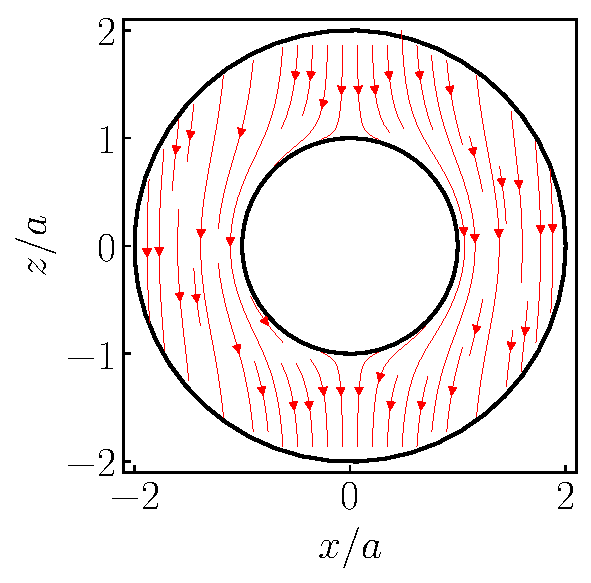
\includegraphics[width=0.7\textwidth]{prob3.pdf}
   \caption{Electric field lines between concentric spheres with the specified boundary conditions and $b = 2a$.}
\end{figure}



}



\end{document}
